\documentclass[tikz,border=2mm]{standalone}
\usepackage{tikz}
\begin{document}
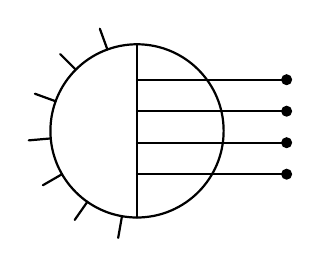
\begin{tikzpicture}[line cap=round,line join=round,thick]

% parameters
\def\R{1.1}          % circle radius
\def\tooth{0.28}     % tooth length
\def\dotr{2pt}       % end-dot radius
\def\L{1.9}          % length of right-side circuit lines

% main circle
\draw (0,0) circle (\R);

% center divider
\draw (0,-\R) -- (0,\R);

% teeth only on the LEFT semicircle (angles 110..250)
\foreach \a in {110,135,160,185,210,235,260}{
  \draw (\a:\R) -- (\a:{\R+\tooth});
}

% circuit lines + end dots (adjust y–positions as you like)
\foreach \y in {0.65,0.25,-0.15,-0.55}{
  \draw (0,\y) -- (\L,\y);
  \fill (\L,\y) circle (\dotr);
}

\end{tikzpicture}
\end{document}
